\section{From a variance bound to volume}
\label{sec:reduction}

We first deduce Theorem~\ref{thm:main} from the variance bound below.
For a probability measure $\mu$, write
$\E_\mu f=\int f\,d\mu$ and
$\Var_\mu(f)=\E_\mu(f-\E_\mu f)^2$.

\begin{proposition}[Variance bound]\label{prop:variance}
Let $n\ge2$, $N\ge1$, $q\ge2$ be an even integer, and $\eps>0$.
Let $p_1,\ldots,p_N\in\R^n\setminus\{0\}$ and $h_1,\ldots,h_N>0$.
Set
\begin{equation}\label{eq:potential}
 \psi_i(x)=\left(\frac{\langle p_i,x\rangle}{h_i}\right)^q,
 \qquad V(x)=\frac{\eps}{2}|x|^2+\sum_{i=1}^N\psi_i(x),
 \qquad d\mu=Z^{-1}e^{-V(x)}\,dx,
\end{equation}
where $Z=\int_{\R^n}e^{-V(x)}\,dx$. For all real $b_1,\ldots,b_N$,
\begin{equation}\label{eq:variance}
 \Var_\mu\left(\sum_{i=1}^N b_i\psi_i\right)
 \le\sum_{i=1}^N b_i^2\E_\mu\psi_i.
\end{equation}
\end{proposition}

Here the Gaussian term makes $Z$ finite, even if the vectors $p_i$
do not span $\R^n$. All polynomial moments are finite. The proof of
Proposition~\ref{prop:variance} occupies Sections~\ref{sec:moment}--\ref{sec:variance}.


The proof will establish the dual estimate
\[
 \sum_{i=1}^N\frac{(\E_\mu u\psi_i)^2}{\E_\mu\psi_i}
 \le \E_\mu u^2
 \qquad\text{for every centered even }u\in L^2(\mu).
\]
Here centered means $\E_\mu u=0$, and the denominators are positive
because each $p_i\ne0$ and $\mu$ has a positive density.
Applied to $u=\sum_i b_i\psi_i-\E_\mu\sum_i b_i\psi_i$, this gives
\eqref{eq:variance} by Cauchy--Schwarz.  We first prove the dual estimate
on a class of smooth compactly supported tests, then use density to
reach every such $u$.  This explains the roles of the density and
tensor lemmas in the analytic proof.

\begin{proof}[Proof of Theorem~\ref{thm:main} from Proposition~\ref{prop:variance}]
Suppose first that $n\ge2$. Fix nonzero spanning vectors
$p_1,\ldots,p_N$ and positive endpoint widths $h_i^0,h_i^1$. For
$t\in[0,1]$, define
\[
 h_i(t)=(h_i^0)^{1-t}(h_i^1)^t,\qquad
 P(t)=\{x:|\langle p_i,x\rangle|\le h_i(t)\text{ for all }i\}.
\]
The spanning condition makes each $P(t)$ bounded; positivity of the
widths gives nonempty interior. Use these widths in \eqref{eq:potential}
and denote the resulting integral by $Z_{q,\eps}(t)$.
For fixed $q,\eps$, its first two derivatives may be taken under the
integral: on a compact interval of $t$, the differentiated integrands
are bounded by a polynomial times $e^{-\eps|x|^2/2}$.
With $b_i=-q\log(h_i^1/h_i^0)$ one has
\[
 \dot V=\sum_i b_i\psi_i,\qquad
 \ddot V=\sum_i b_i^2\psi_i,
\]
and hence
\[
 \frac{d^2}{dt^2}\log Z_{q,\eps}(t)
 =\Var_{\mu_t}(\dot V)-\E_{\mu_t}\ddot V\le0
\]
by Proposition~\ref{prop:variance}. Therefore
\begin{equation}\label{eq:partition-concavity}
 Z_{q,\eps}(\lambda)\ge
 Z_{q,\eps}(0)^{1-\lambda}Z_{q,\eps}(1)^\lambda.
\end{equation}

Keep $\eps>0$ fixed and let $q$ tend to infinity through even integers.
For each fixed $t$, the integrands converge almost everywhere to
$e^{-\eps|x|^2/2}\mathbf1_{P(t)}$. The exceptional set lies in the
finitely many hyperplanes $\langle p_i,x\rangle=\pm h_i(t)$ and
has measure zero. The common integrable bound
$e^{-\eps|x|^2/2}$ gives
\[
 Z_{q,\eps}(t)\longrightarrow
 \int_{P(t)}e^{-\eps|x|^2/2}\,dx.
\]
Apply this at $t=0,\lambda,1$ in \eqref{eq:partition-concavity}, then
let $\eps\downarrow0$. Monotone convergence gives
\begin{equation}\label{eq:slabs}
 |P(\lambda)|\ge |P(0)|^{1-\lambda}|P(1)|^\lambda.
\end{equation}

\begin{figure}[tb]
  \centering
  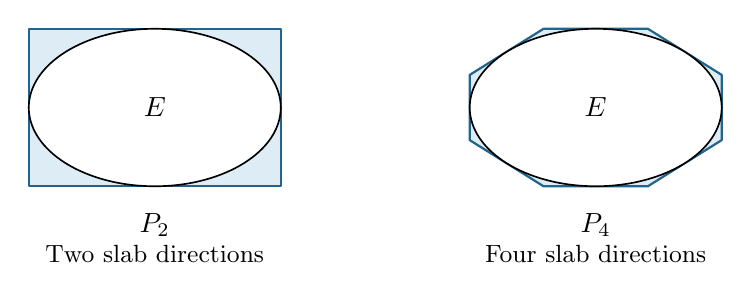
\begin{tikzpicture}[x=1cm,y=1cm,line join=round]
    \definecolor{slabblue}{RGB}{34,100,139}
    \definecolor{slabfill}{RGB}{222,237,245}
    \begin{scope}[xshift=-2.8cm]
      \filldraw[fill=slabfill,draw=slabblue,line width=0.8pt]
        (-1.6,-1) rectangle (1.6,1);
      \filldraw[fill=white,draw=black,line width=0.6pt]
        (0,0) ellipse [x radius=1.6,y radius=1];
      \node at (0,0) {$E$};
      \node[anchor=north] at (0,-1.22) {$P_2$};
      \node[anchor=north,font=\small] at (0,-1.62)
        {Two slab directions};
    \end{scope}
    \begin{scope}[xshift=2.8cm]
      \foreach \k in {0,...,7} {
        \coordinate (p\k) at
          ({1.6*cos(22.5+45*\k)/cos(22.5)},
           {sin(22.5+45*\k)/cos(22.5)});
      }
      \filldraw[fill=slabfill,draw=slabblue,line width=0.8pt]
        (p0) \foreach \k in {1,...,7} {-- (p\k)} -- cycle;
      \filldraw[fill=white,draw=black,line width=0.6pt]
        (0,0) ellipse [x radius=1.6,y radius=1];
      \node at (0,0) {$E$};
      \node[anchor=north] at (0,-1.22) {$P_4$};
      \node[anchor=north,font=\small] at (0,-1.62)
        {Four slab directions};
    \end{scope}
  \end{tikzpicture}
  \caption{Finite outer approximations of an ellipse $E$. Adding slab
  directions gives $P_2\supset P_4\supset E$; the subscripts here count
  slab directions. Using nested finite spanning direction
  sets with dense union, the same construction recovers $\mathcal W[f]$ from any
  positive continuous even function $f$ on the sphere; $f$ need not be a
  support function.}
  \label{fig:slab-exhaustion}
\end{figure}


Figure~\ref{fig:slab-exhaustion} illustrates how additional slab
directions refine an outer approximation.  To pass to all directions,
let $K,L$ be as in Theorem~\ref{thm:main}. Choose nested finite
sets $D_m\subset S^{n-1}$ that contain the coordinate vectors and
whose union is dense in the sphere. Define
\[
 P_m(t)=\bigcap_{p\in D_m}
 \{x:|\langle p,x\rangle|\le h_K(p)^{1-t}h_L(p)^t\}.
\]
The bodies $P_m(t)$ decrease with $m$ and are all contained in the bounded
body $P_1(t)$. By continuity of the support functions and their
evenness,
\[
 \bigcap_m P_m(t)=\mathcal W[h_K^{1-t}h_L^t].
\]
Indeed any point satisfying the dense set of inequalities satisfies
all of them by continuity in the direction. Conversely, the Wulff
inequalities imply the absolute-value constraints by evenness.
At $t=0,1$ these intersections are $K,L$, respectively, by the
supporting-half-space characterization of a convex body.
Continuity of measure from above, applied at $0,\lambda,1$ in
\eqref{eq:slabs}, proves \eqref{eq:main}.

Finally, in dimension one write $K=[-a,a]$ and $L=[-b,b]$ with
$a,b>0$. Their Wulff interpolation is the interval with radius
$a^{1-\lambda}b^\lambda$, whose length is
$(2a)^{1-\lambda}(2b)^\lambda$. Thus \eqref{eq:main} is equality.
The endpoints $\lambda=0,1$ are equality in every dimension.
\end{proof}
